%% Bemærk:
%%          Resten af rapporten følger en stil hvor indledninger skrives
%%          med \sffamlily-typen. Denne stil bør ikke bruges her, da dette ikke er \section
%%
{
Ved udtrækning af regioner sætter vi en værdi for, hvor stor en region skal
være, for at blive tage i betragtning. I dette afsnit vil vi teste, hvor stor
en region skal være for at vi vil tage den med. Problematikken med for små
regioner er illustreret i maleriet i figur \ref{alt_med}. Her er alle de grønne
kasser regioner, som vores naive algoritme mener er interessante, og da
alle regioner er taget med, bliver 939 regioner vurderet til at ligge i
snittet.

\begin{figure}[¡h]
    \setlength\fboxsep{0pt}
    \setlength\fboxrule{0.5pt}
    \begin{center}
        \fbox{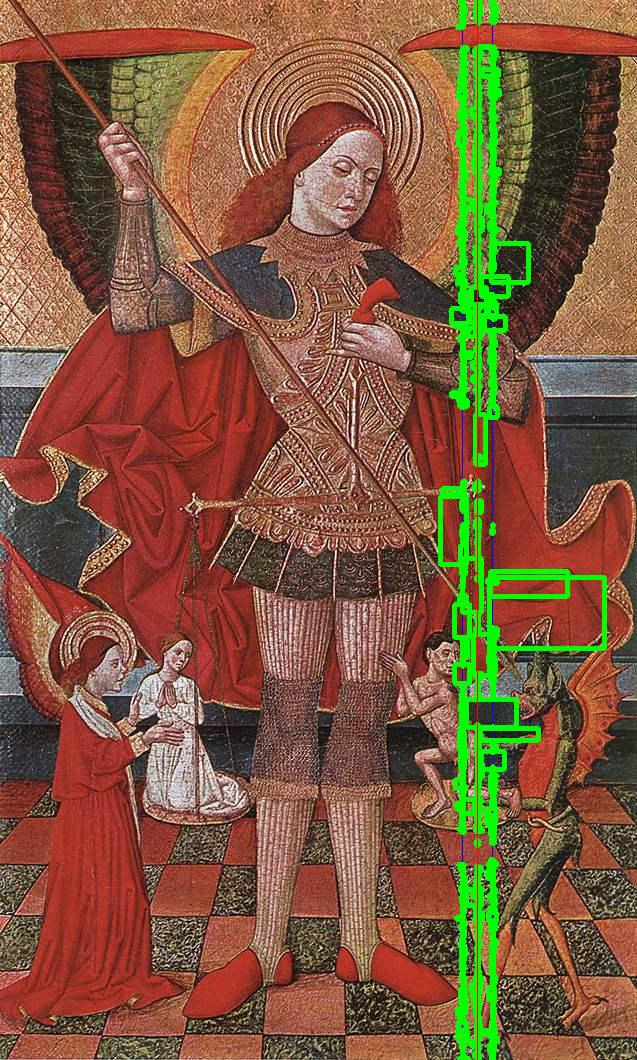
\includegraphics[angle=0,width=0.45\textwidth]{afsnit/afprovning/billeder/stoerelse/alt_med.png}}
    \end{center}
    \caption{Maleri, hvor regioner i alle størrelser er godtaget. Der er
	fundet $939$ interessante regioner.}
	\label{alt_med}
\end{figure}

For at teste hvilken størrelse, vi bør godtage, er der fremstillet et
testbillede i figur \ref{original_stoerelse}, hvor ni regioner er opstillet,
således at de alle ligger i samme snit. Den øverste region er den mindste, og
regionernes størrelse stiger gradvist ned langs snittet.

I hver af de andre fem testbilleder i figur \ref{stoerelse_sammenlining}, er
tærskelværdierne gradvist sat op. De regioner, der godtages, er repræsenteret med grønne kasser. 
Vi mener, at der bliver taget for mange regioner med i billede \ref{0,0}, \ref{0,005}, \ref{0,001} og
\ref{0,0015}. I billedet \ref{0,002} vurderer vi, at det kun er regioner
af en vis størrelse, som er blevet udvalgt, og vi har derfor
valgt at sætte tærskelværdien til $0.002$.

\begin{figure}[!h]
    \setlength\fboxsep{0pt}
    \setlength\fboxrule{0.5pt}
    \centering
    \subfloat[Det originale billede.]{
        \fbox{
\includegraphics[angle=0,width=0.45\textwidth]{afsnit/afprovning/billeder/stoerelse/stoerelse.png}}
       \label{original_stoerelse}}
    \subfloat[Tærskelværdien sat til $0$.]{
        \fbox{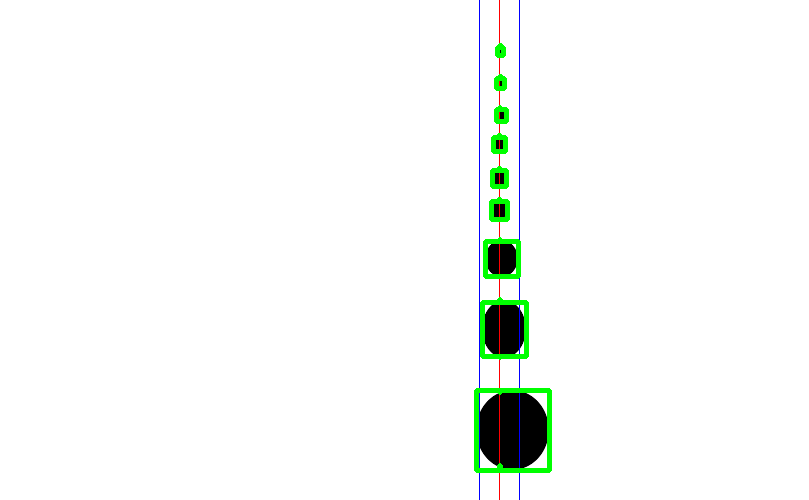
\includegraphics[angle=0,width=0.45\textwidth]{afsnit/afprovning/billeder/stoerelse/0.png}}
       \label{0,0}}\\
    \subfloat[Tærskelværdien sat til $0.0005$.]{
        \fbox{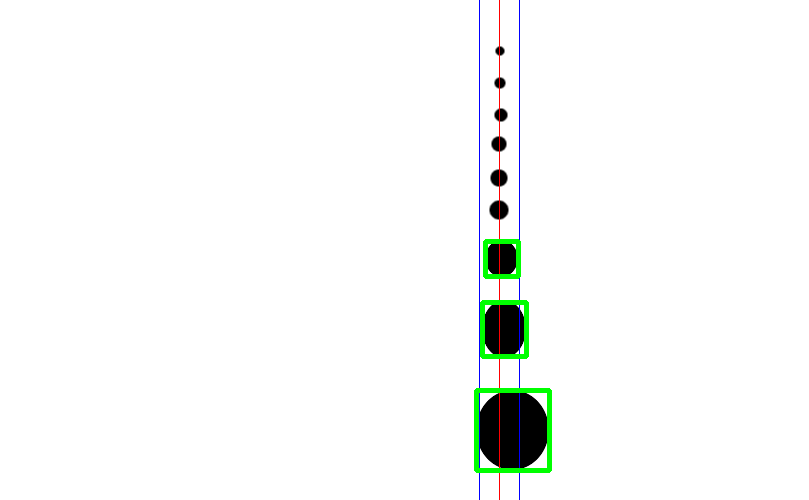
\includegraphics[angle=0,width=0.45\textwidth]{afsnit/afprovning/billeder/stoerelse/0,0005.png}}
       \label{0,005}}
    \subfloat[Tærskelværdien sat til $0.001$.]{
        \fbox{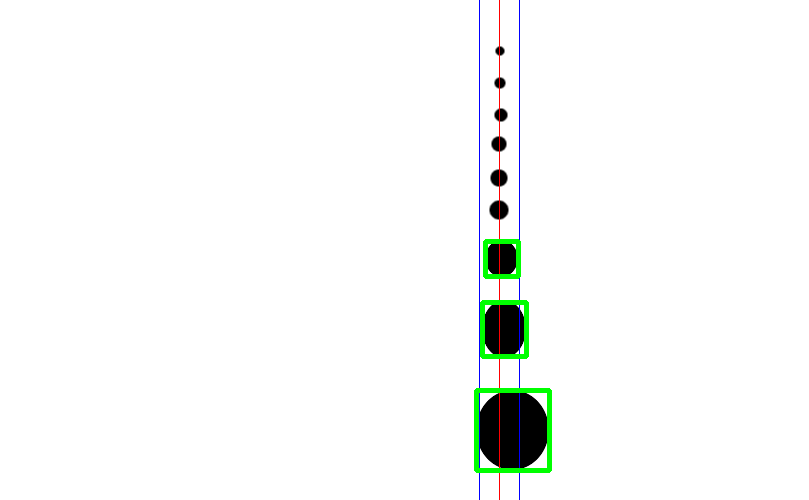
\includegraphics[angle=0,width=0.45\textwidth]{afsnit/afprovning/billeder/stoerelse/0,001.png}}
       \label{0,001}}\\
    \subfloat[Tærskelværdien sat til $0.0015$.]{
        \fbox{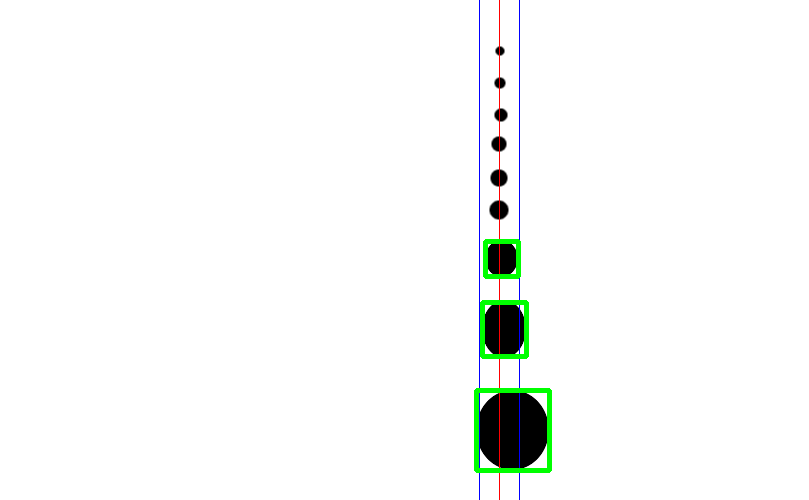
\includegraphics[angle=0,width=0.45\textwidth]{afsnit/afprovning/billeder/stoerelse/0,0015.png}}
       \label{0,0015}}
    \subfloat[Tærskelværdien sat til $0.002$.]{
        \fbox{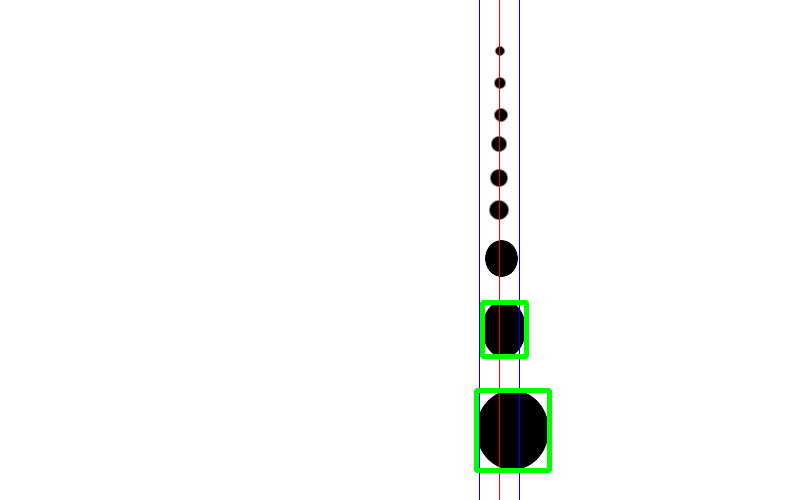
\includegraphics[angle=0,width=0.45\textwidth]{afsnit/afprovning/billeder/stoerelse/0,002.png}}
       \label{0,002}}
    \caption{Testbillede, med ni regioner som bliver større og større.
	Det originale billede, samt fem forskellige tærskelværdier, er afbilledet.}
    \label{stoerelse_sammenlining}
\end{figure}
}
